\section{Pianificazione}
Alla luce delle scadenze presentate nella \hyperlink{scadenze}{sottosezione 2.5}, la pianificazione di progetto viene suddivisa nelle seguenti fasi:
\begin{enumerate}
	\item \textbf{Analisi};
	\item \textbf{Consolidamento dei requisiti};
	\item \textbf{Progettazione architetturale};
	\item \textbf{Progettazione di dettaglio e codifica};
	\item \textbf{Validazione e collaudo}.
\end{enumerate}
Ogni fase viene suddivisa in attività\glosp che verranno realizzate durante il 
periodo stabilito per la fase stessa. 
\subsection{Analisi}
\textit{Periodo: dal 2018-11-16 al 2019-01-14}\\
L'inizio del periodo di questa fase coincide con la data di formazione dei 
gruppo e la fine coincide con la data di consegna dei documenti relativi alla 
revisione dei requisiti. Questa fase è stata scomposta nelle seguenti sotto attività:
\begin{itemize}
	\item \textbf{Individuazione degli strumenti}: questa attività consiste nel 
	determinare quali strumenti il gruppo deve utilizzare per la comunicazione, per 
la stesura dei documenti e per il versionamento, lo sviluppo e la verifica del 
software; 
	\item \textbf{Norme di Progetto}: sono definite tutte le regole utili per lo svolgimento del progetto, relative al prodotto da realizzare e ai processi da adottare. Il documento \textit{Norme di Progetto} viene redatto dal Responsabile di progetto e dall'Amministratore;
	\item \textbf{Studio di fattibilità}: in questa attività gli Analisti effettuano uno studio sommario dei capitolati in modo da determinare quale di essi verrà scelto. Questa attività e da considerarsi bloccante per l'attività di \textit{Analisi dei Requisiti};
	\item \textbf{Analisi dei Requisiti}: durante questa attività vengono 
	identificati ed analizzati i requisiti del capitolato scelto nell'attività 
	di \textit{Studio di fattibilità} e il relativo documento viene composto dagli Analisti;
	\item \textbf{Piano di Progetto}: il Responsabile pianifica il 
	lavoro del gruppo 8Lab Solutions, inteso come suddivisione di compiti, 
	risorse e attività. Inoltre viene calcolato il preventivo per la realizzazione 
	del progetto. Questa attività comporta anche la stesura 
	del documento \textit{Piano di Progetto};
	\item \textbf{Piano di Qualifica}: in questà attività si individuano le 
	metodologie attraverso le quali si garatisce la qualità del prodotto. A supporto di ciò viene redatto il documento \textit{Piano di Qualifica} da parte degli Analisti; 
	\item \textbf{Glossario}: vengono individuati tutti i termini che possono risultare ambigui e 
	vengono definiti nel documento \textit{Glossario} che viene 
	redatto durante tutta la fase di analisi dei requisiti.
\end{itemize}

\begin{figure}[H]
	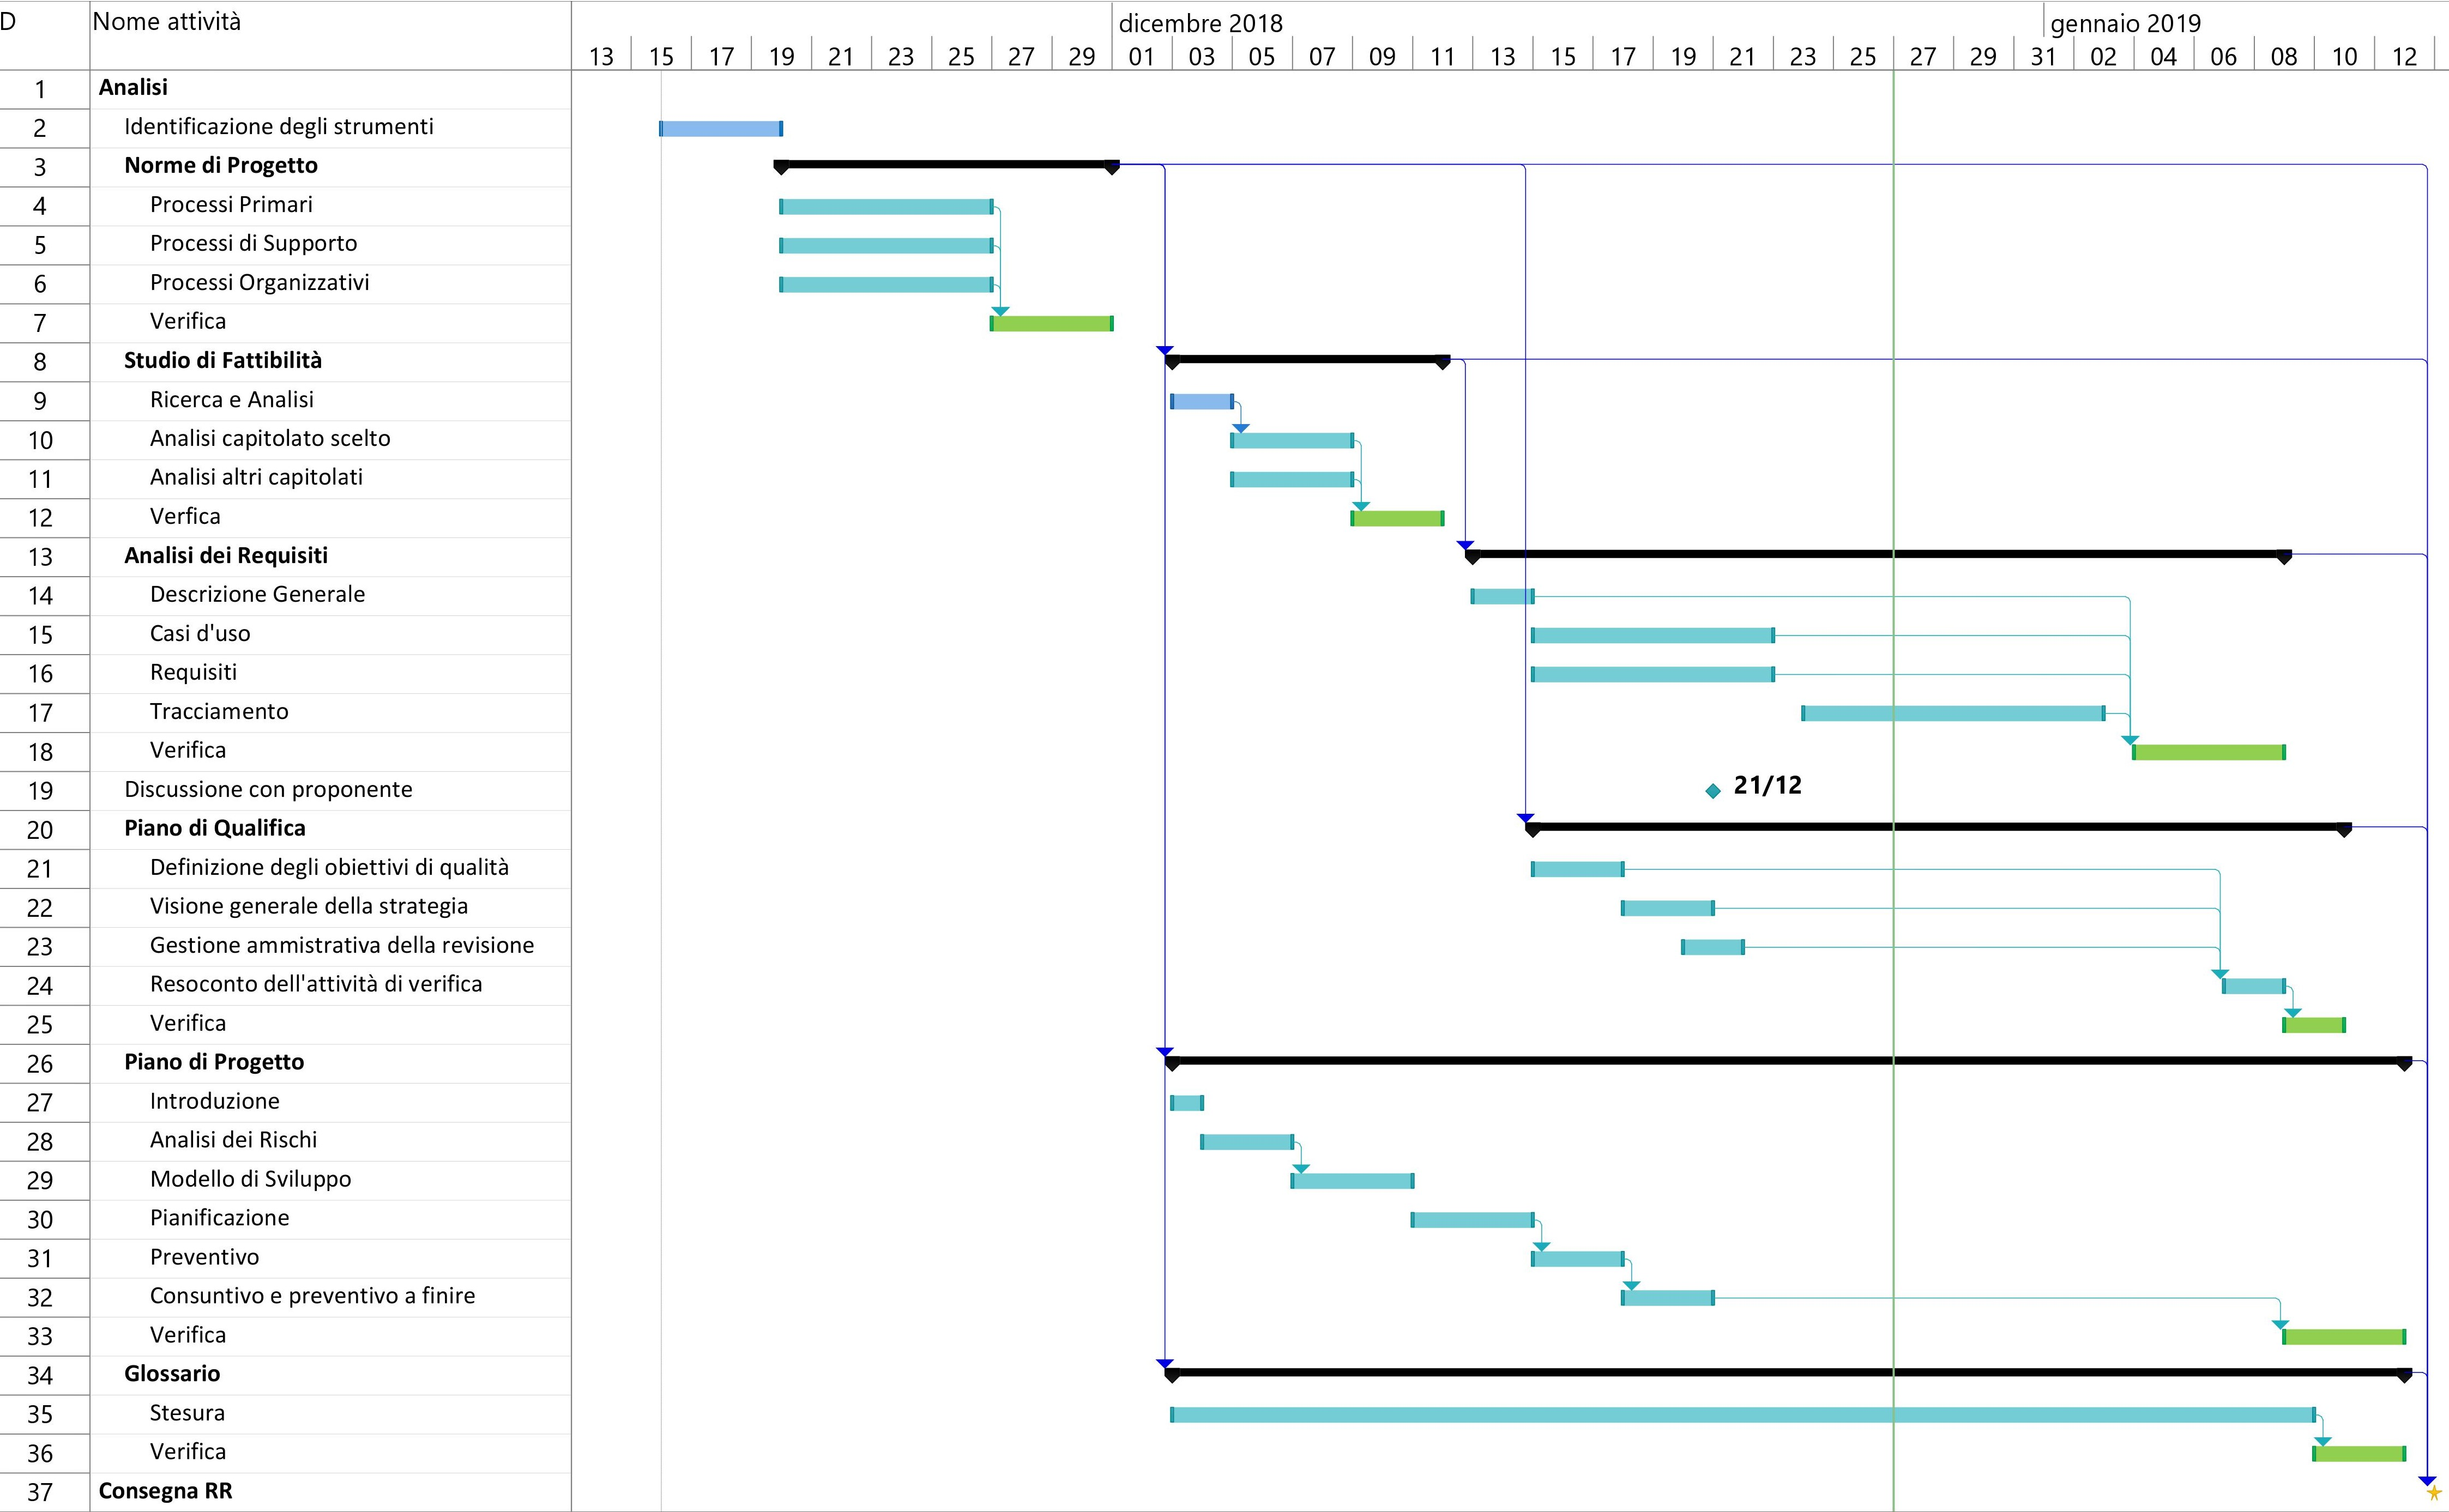
\includegraphics[width=0.99\linewidth]{res/images/gantt_analisi1.jpg}
	\caption{Diagramma di Gantt della fase di Analisi}
\end{figure}



\subsection{Consolidamento dei requisiti}
\textit{Perdiodo: dal 2019-01-14 al 2019-01-21} \\
Questa fase comincia con la fine della fase di \textit{Analisi} e termina il giorno della presentazione della \textit{Revisione dei Requisiti}. Le attività di questa fase sono:
\begin{itemize}
	\item \textbf{Consolidamento}: questa attività ha lo scopo di consolidare e migliorare i requisiti ottenuti nella fase precendente;
	\item \textbf{Incremento e Verifica}: se necessario vengono migliorati i documenti prodotti nella fase precendente.
\end{itemize}
Inoltre durante questa fase ogni componente del gruppo dovrà dedicare almeno 15 
ore di studio e approfondimento delle tecnologie necessarie alle prossime fasi 
e alla realizzazione del prodotto. Questa attività verrà gestita in modo 
autonomo dai membri del gruppo, quindi non sarà riportata nel diagramma di 
Gantt~\ref{fig:gantt_con} sottostante.

\begin{figure}[H]
	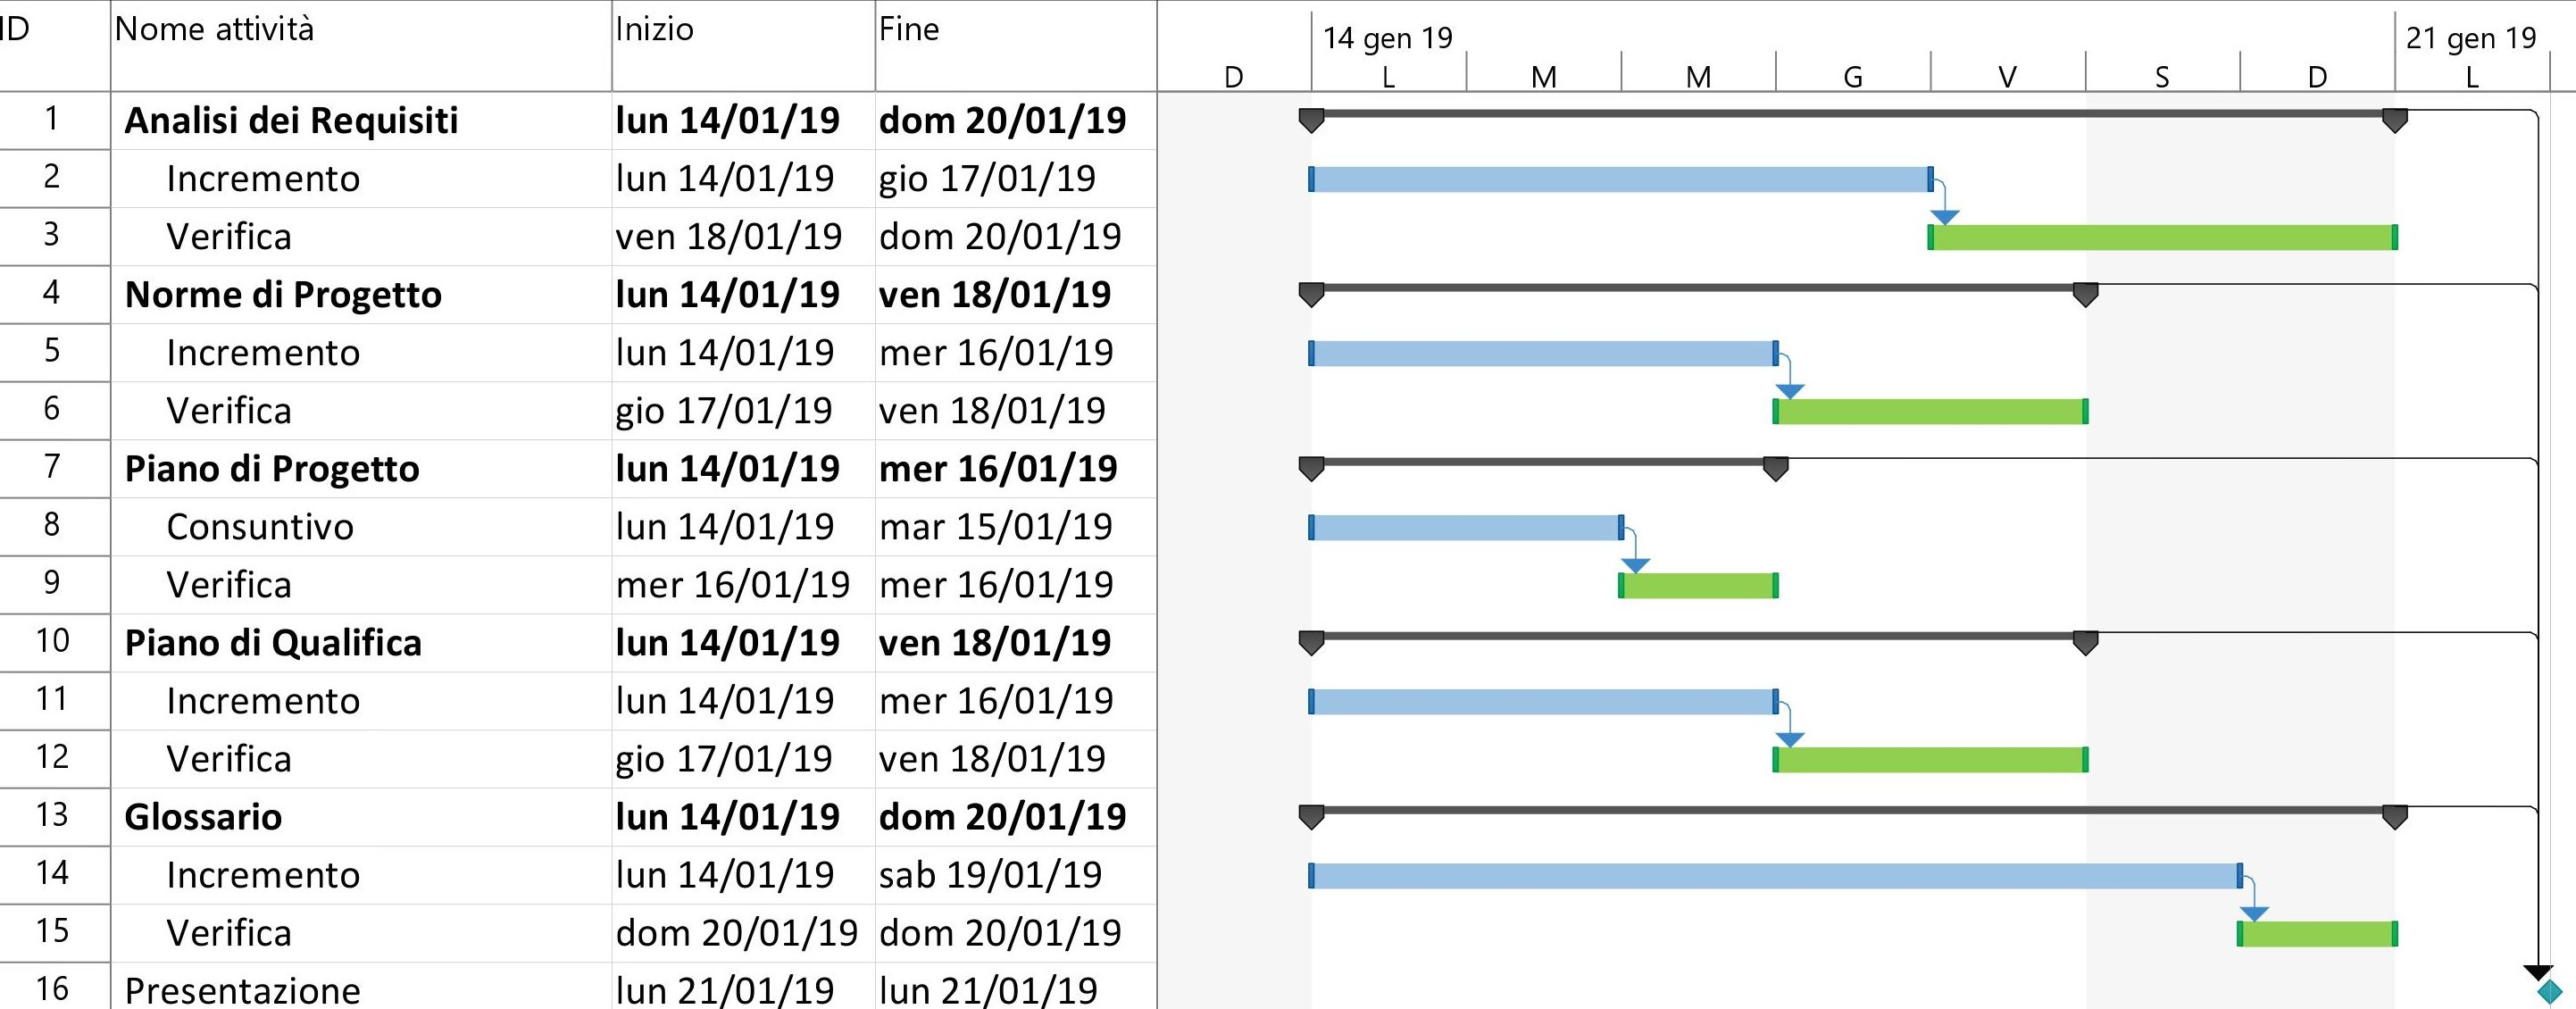
\includegraphics[width=0.99\linewidth]{res/images/gantt_cons.jpg}
	\caption{Diagramma di Gantt della fase di Consolidamento dei requisiti}
	\label{fig:gantt_con}
\end{figure}

%-----------------Sottosezione Progettazione Architetturale---------------------
\subsection{Progettazione architetturale}
\textit{Periodo: dal 2019-01-21 al 2019-03-08} \\
Questa fase comincia il giorno dopo la presentazione e la fine coincide con la data di consegna \textit{Revisione di 
Progettazione}. In questo periodo verrà individuata una soluzione architetturale 
tale per cui i requisiti richiesti vengano soddisfatti.
\begin{itemize}
	\item \textbf{Specifica Tecnica}: viene redatto il documento 
	\textit{Specifica Tecnica} nel quale vengono individuati i design 
	pattern\glosp che verranno adottati per lo sviluppo. Inoltre il documento 
	include il tracciamento dei requisiti.\\
	Infine viene codificato il \textbf{\textit{Proof of Concept}}\glosp il 
	quale viene presentato o condiviso tramite repository al committente e 
	proponente in una data da definirsi.
	\item \textbf{Incremento e Verifica}: se necessario vengono migliorati i 
	documenti prodotti nelle fasi precedenti.
\end{itemize}

\begin{figure}[H]
	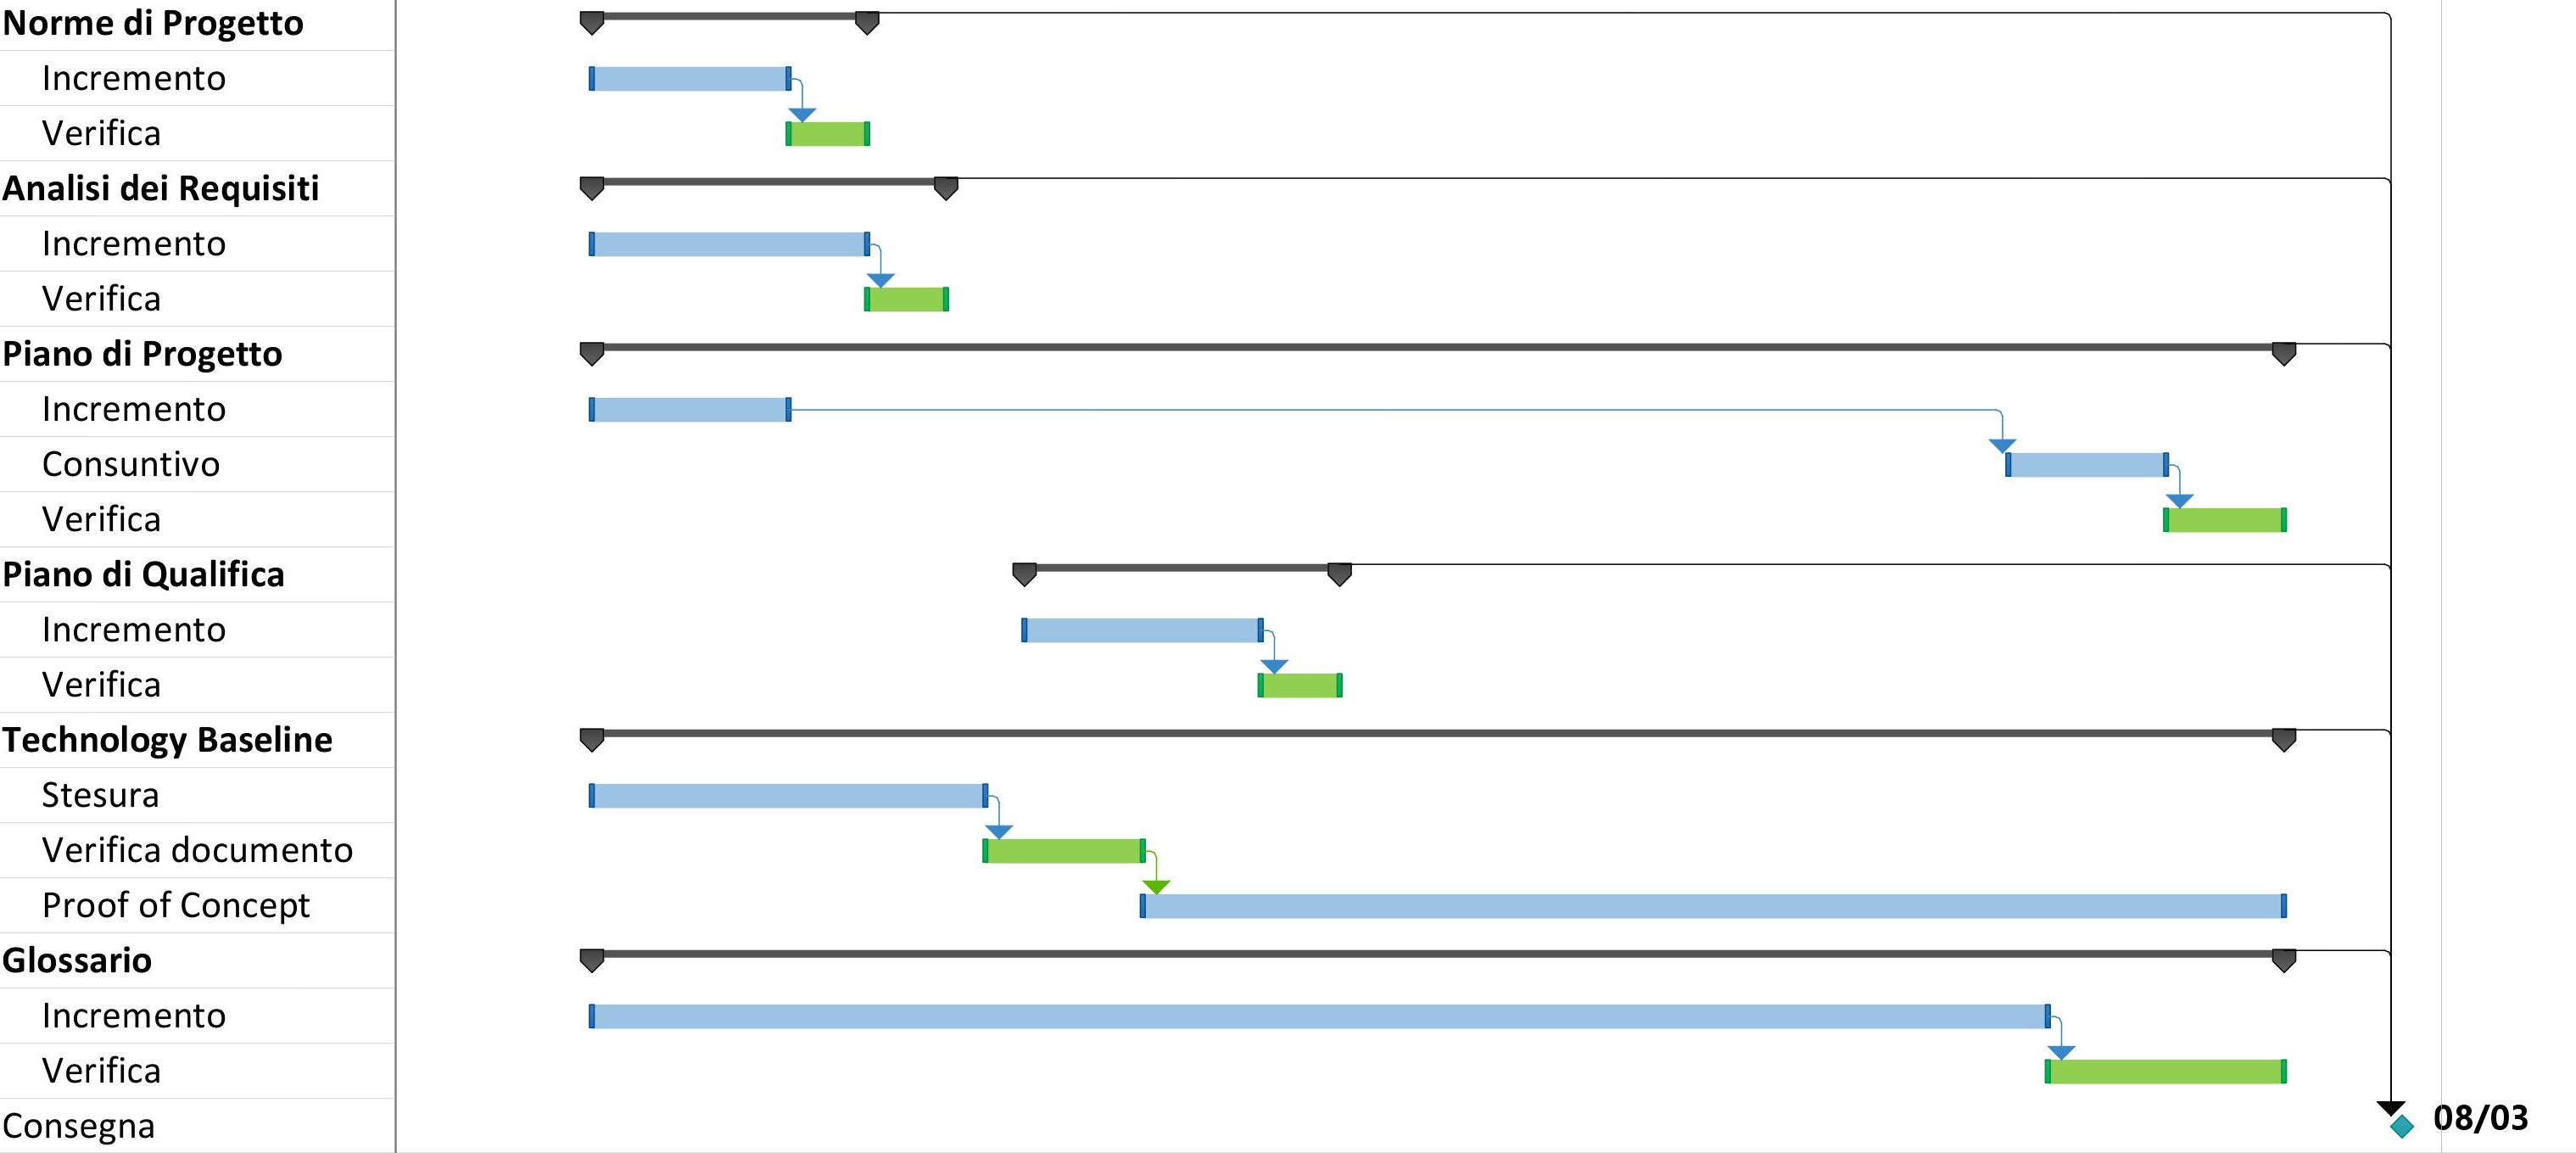
\includegraphics[width=0.99\linewidth]{res/images/gantt_pa.jpg}
	\caption{Diagramma di Gantt della fase di Progettazione architetturale}
\end{figure}


%-------------------Sottosezione Progettazione di Dettaglio---------------------
\subsection{Progettazione di dettaglio e codifica}
\textit{Periodo: dal 2019-03-15 al 2019-04-12}
L'inizio di questa fase è il giorno della scadenza della \textit{Revisione di 
Progettazione} e la data di fine coincide con la data di consegna dei documenti 
in vista della \textit{Revisione di Qualifica}. Le attività di questa fase sono:
\begin{itemize}
	\item \textbf{Definizione di Prodotto}: a seguito della \textit{Specifica 
	Tecnica} l'architettura individuata in essa viene scomposta nei suoi 
	componenti per esseri analizzati nel dettaglio in modo tale da fornire i 
	dettagli necessari alla codifica e alla verifica dei componenti. A supporto 
	di ciò viede redatto il documento \textit{Definizione di Prodotto};
	\item \textbf{Codifica}: questa attività consiste nella scrittura del 
	codice e della sua verifica con modalità e strumenti definiti nel 
	\textit{Piano di Qualifica v2.0.0}
	\item \textbf{Manuale Utente}: viene redatto il documento \textit{Manuale 
	Utente} atto a fornire istruzioni e indicazioni per l'utilizzo del prodotto;
	\item \textbf{Incremento e Verifica}: se necessario vengono migliorati i 
	documenti prodotti nelle fasi precedenti.
\end{itemize}


\begin{figure}[H]
	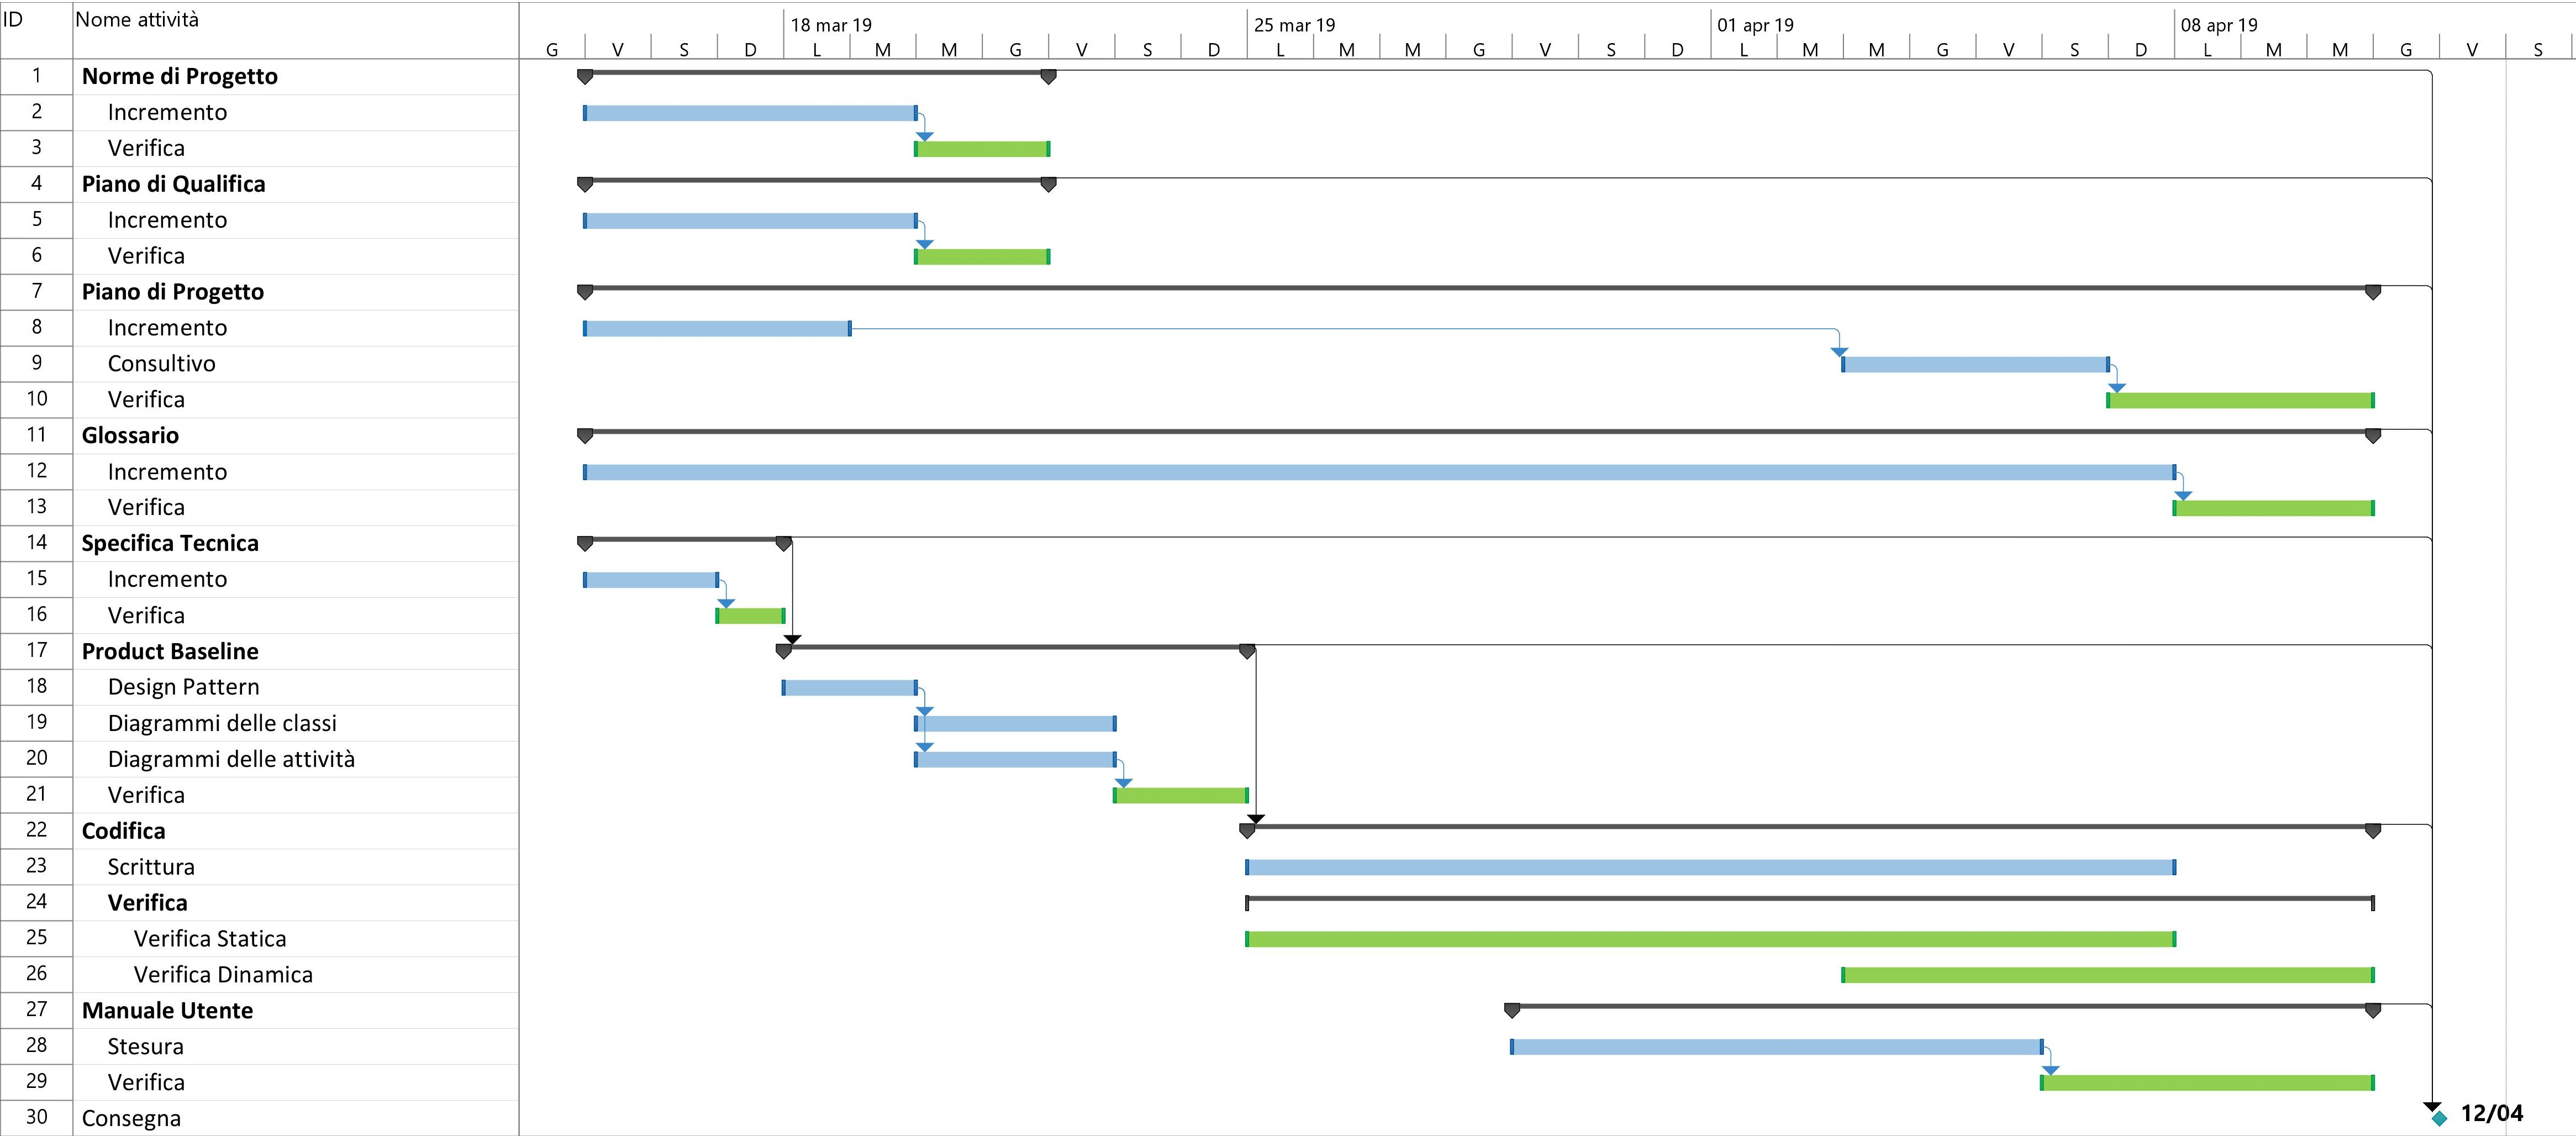
\includegraphics[width=0.99\linewidth]{res/images/gantt_pd.jpg}
	\caption{Diagramma di Gantt della fase di Progettazione di dettaglio e codifica}
\end{figure}
\pagebreak

\subsection{Validazione e collaudo}
\textit{Periodo: dal 2019-04-12 al 2019-05-17 } \\
L'inizio di questa fase coincide col la data di consegna dei documenti per la 
\textit{Revisione di Qualifica}, mentre la data di fine coincide con la 
consegna in vista della \textit{Revisione di Accettazione}. Durante questo periodo 
si eseguiranno ulteriori attività di validazione e verifica. Le attività 
previste sono: 
\begin{itemize}
	\item \textbf{Validazione e Collaudo}: per la parte di collaudo si 
	eseguiranno ulteriori test sul prodotto, in modo da garantirne la 
	correttezza e stabilità. Per la parte di validazione, verrà 
	valutata la coerenza del prodotto e dei requisiti specificati nel documento 
	\textit{Analisi dei Requisiti} nella sua ultima versione;
	\item \textbf{Manuale Sviluppatore}: viene redatto il documento \textit{Manuale Sviluppatore} atto a fornire tutte le informazioni necessarie al mantenimento, manutenzione e ampliamento del prodotto finale;
	\item \textbf{Incremento e Verifica}: se necessario vengono migliorati i 
	documenti prodotti nelle fasi precedenti.
\end{itemize}
\begin{figure}[H]
	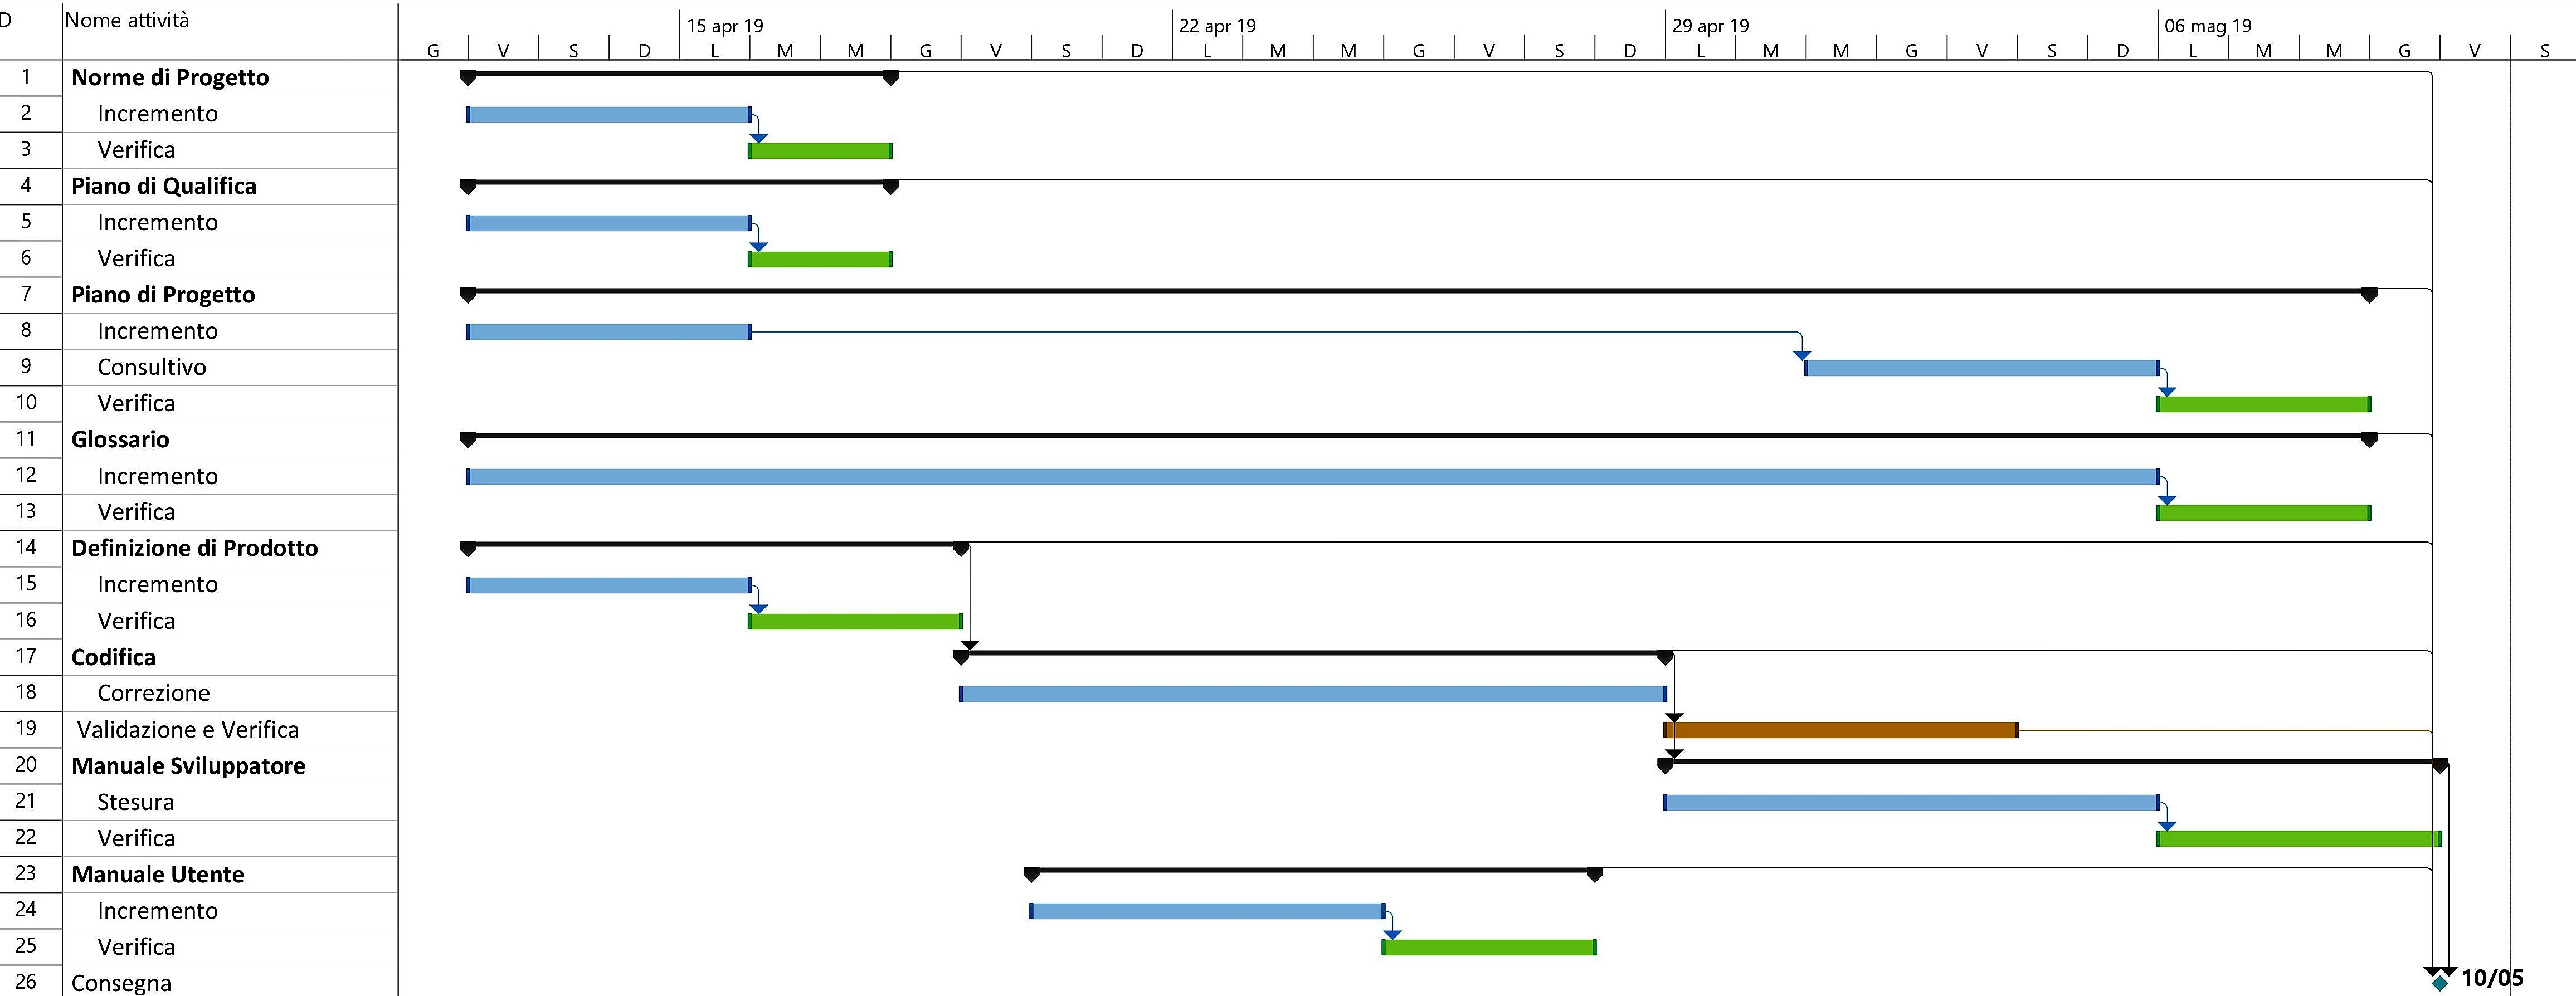
\includegraphics[width=0.99\linewidth]{res/images/gantt_val.jpg}
	\caption{Diagramma di Gantt della fase di Validazione e collaudo}
\end{figure}